\documentclass[dvipsnames]{beamer}

\usepackage[slovene]{babel}
\usepackage[T1]{fontenc}
\usepackage[utf8]{inputenc}
\usepackage{lmodern}

\usepackage{amssymb}
\usepackage{amsmath}

\usepackage{xcolor}

\usepackage{enumerate}
\usepackage{graphicx}

\usetheme{Ilmenau}
\usecolortheme{beaver}

\setbeamercolor{block title}{bg=darkred,fg=structure.fg!20!bg!50!bg}
%\setbeamercolor{block body}{bg=white}

% commands
\newcommand{\graf}[1][G]{\ensuremath{#1 = (V(#1), E(#1))}}
\newcommand{\vozlisca}[1][G]{\ensuremath{V(#1)}}
\newcommand{\povezave}[1][G]{\ensuremath{E(#1)}}
\newcommand{\bd}{\ensuremath{|\,}}
\newcommand{\ed}{\ensuremath{\,|}}
% operatorji
\DeclareMathOperator {\stopnja} {deg}


\title{Problem londonskega stolpa}
\author[Ines Meršak]{Ines Meršak \\[5px] mentor: prof.~dr.~Sandi Klavžar}
\date{TODO.~2016}

\begin{document}
    
\begin{frame}[plain]
    \titlepage
\end{frame}

%\begin{frame}
%    Kratka predstavitev:
%    \begin{itemize}
%        \item klasičen problem londonskega stolpa - opis igre
%        \item osnovne definicije teorije grafov
%        \item klasičen problem londonskega stolpa - lastnosti grafa (Hamiltonova pot, etc.)
%        \item posplošen londonski stolp - definicija, povezanost, planarnost
%        \item primeri uporabe v psihologiji
%    \end{itemize}
%\end{frame}

\section{Klasični problem londonskega stolpa}
\begin{frame}{Klasični problem londonskega stolpa (Shallice)}
    \begin{figure}
        \centering
        
\includegraphics[height=100pt]{../img/london-tower.png}
    \end{figure}
    \begin{itemize}
        \item izumljen leta 1982
        \item 3 enako velike krogle različnih barv
        \item 3 palice različnih velikosti
        \item cilj igre je priti iz trenutnega stanja v neko dano stanje z minimalnim številom potez
    \end{itemize}
\end{frame}

%\begin{frame}{Osnovne definicije teorije grafov}
%    \begin{itemize}
%        \item graf $ G = (V, E) $
%        \item \alert{soseščina} vozlišča $u$: $N(u) = \{x \in V;\ ux \in E\}$
%        \item \alert{stopnja} vozlišča $u$: $\stopnja u  = \lvert N(u) \rvert$
%        \item \alert{sprehod} v grafu je zaporedje vozlišč $v_1,\ldots, v_k$, da za vsak $i$ velja $v_i v_{i+1} \in E$
%        \item graf je \alert{povezan}, če za poljuben par vozlišč obstaja sprehod med njima
%        \item \alert{razdalja} $d_G(u,v)$ je najmanjše možno število povezav na nekem sprehodu, ki se začne v vozlišču $u$ in konča v vozlišču $v$
%        \item \alert{premer} grafa je največja minimalna razdalja med pari vozlišč
%    \end{itemize}
%\end{frame}
%
%\begin{frame}
%    \begin{itemize}
%        \item \alert{ravninski} graf je graf, ki ga lahko narišemo v ravnini brez križanja povezav
%        \item pot v grafu, ki vsebuje vsa vozlišča, je \alert{Hamiltonova pot}
%        \item \alert{Hamiltonov cikel} je cikel v grafu, ki poteka skozi vsa vozlišča
%    \end{itemize}
%\end{frame}

\begin{frame}{Primer}
    \begin{figure}
        \centering
        
\includegraphics[height=150pt]{../img/london-tower.png}
    \end{figure}
\end{frame}

\begin{frame}{Graf klasičnega problema londonskega stolpa}
%    Označimo krogle s številkami 1, 2, 3, pri čemer je npr.\ krogla 1 modra, krogla 2 rdeča, krogla 3 pa rumena. Začetek nove palice bomo nakazali z |, krogle pa bomo naštevali od vrha proti dnu palice.
    
    \begin{figure}
        \centering
        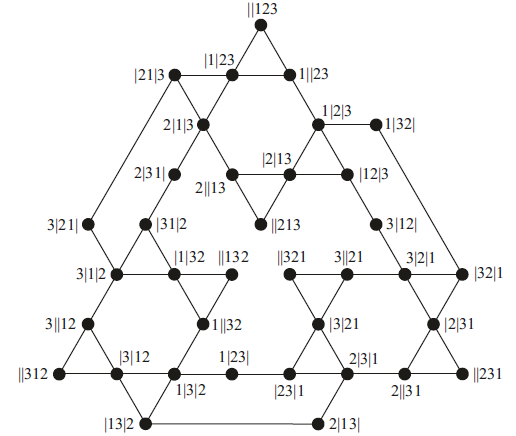
\includegraphics[height=190pt]{../img/tolgraph.png}
    \end{figure}
\end{frame}


\begin{frame}{Lastnosti grafa}
    \begin{itemize}
        \item 36 vozlišč (36 možnih stanj)
        \item po 12 vozlišč stopnje 2, 3, 4
        \item premer grafa je 8
        \item ravninski
    \end{itemize}
   	\begin{block}{Trditev}
   		Klasični londonski graf vsebuje Hamiltonovo pot, ne pa tudi Hamiltonovega cikla.
   	\end{block}
\end{frame}

\begin{frame}
    \begin{figure}
        \centering
        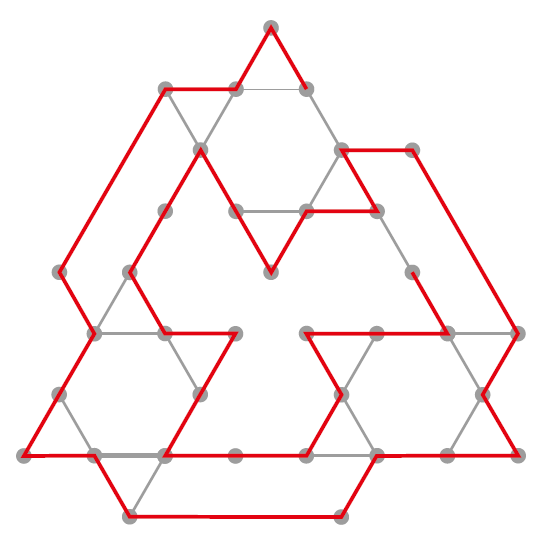
\includegraphics[height=190pt]{../img/tolgraph-ham-path.png}
    \end{figure}
\end{frame}

\begin{frame}
    \begin{figure}
        \centering
        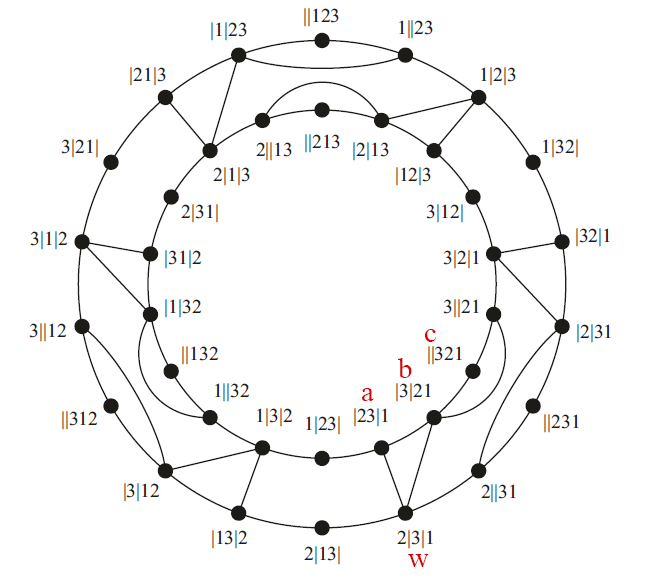
\includegraphics[height=190pt]{../img/tolgraph-ham-cycle.png}
    \end{figure}
\end{frame}

\section{Posplošen londonski stolp}
\begin{frame}{Oznake}
    \begin{itemize}
        \item J.\ R.\ Tunstall je prva predlagala razširitev na 4 krogle s podaljšanimi palicami
        \item $n$ krogel različnih barv, $n \geq 2$
        \item $p$ palic, $p \geq 3$
        \item vsako palico označimo s številom $k \in [p]$, njeno višino pa s $h_k$
        \item veljati mora $n \leq \sum_{k=1}^p h_k$
        \item veljavnost poteze
        \item vsako stanje lahko enolično predstavimo s permutacijo $s \in S_{n+p}$
        \item položaje oštevilčimo od leve palice proti desni, z vrha palice proti dnu
    \end{itemize}
\end{frame}

\begin{frame}{Primer}
    \begin{figure}
        \centering
        
\includegraphics[height=150pt]{../img/london-tower.png}
    \end{figure}
\end{frame}

\begin{frame}{Definicija}
    \begin{block}{Definicija}
        \alert{Londonski graf} $L_h^n$, kjer je $p \geq 3,\ n \geq 2,\ h \in [n]^p,\  \sum_{k=1}^p h_k \geq n$:
        \begin{itemize}
            \item vozlišča: vse permutacije $s \in S_{n+p}$, za katere velja:
            \[\forall k \in [p]:\ 1 \leq s_{n+k} - s_{n+k-1} \leq h_k + 1,\ s_{n+p} = n + p ,\]
            \item povezave: vsaki dve stanji (oz.\ pripadajoči permutaciji), med katerima lahko prehajamo z veljavno potezo, sta povezani
        \end{itemize}
    \end{block}

\end{frame}

\begin{frame}{Povezanost grafa}
    V nadaljevanju bomo privzeli, da so palice urejene po velikosti naraščajoče, velja torej $h_1 \leq h_2 \leq \cdots \leq h_p$.
    
    Potreben pogoj za povezanost londonskega grafa je 
    \[ n \leq \sum_{k=1}^{p-1} h_k. \]
    \begin{block}{Izrek}
        Londonski graf $L_h^n$ je povezan natanko tedaj, ko velja pogoj
        \[ n \leq \sum_{k=1}^{p-1} h_k. \]
    \end{block}
\end{frame}

\begin{frame}{Ravninskost grafa}
    \begin{figure}[h]
        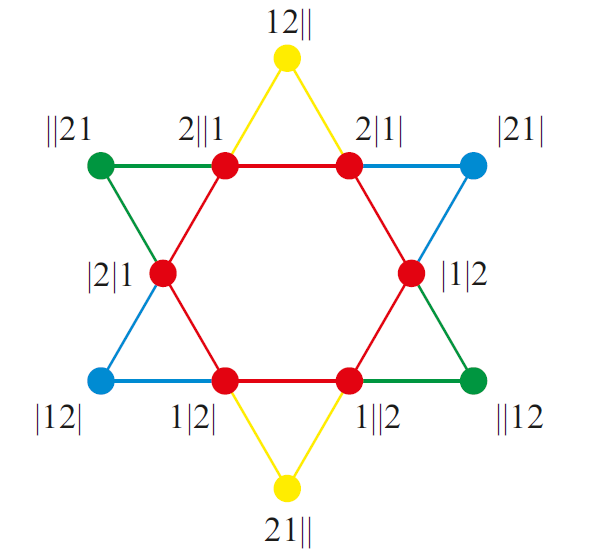
\includegraphics[width=150pt]{../img/tolgraph-2balls.png}
        \caption{Vsi londonski grafi s $p=3$ in $n=2$ so ravninski. Prikazani so: 
            ${\color{Red} L^2_{111}} + 
            {\color{Green}L^2_{112}} + 
            {\color{NavyBlue}L^2_{122}} + 
            {\color{Yellow}L^2_{222}}$.}
    \end{figure}
\end{frame}

\begin{frame}
    Operacija \alert{subdivizije} ohranja ravninskost.
    \begin{block}{Izrek Kuratowskega}
           	Graf G je ravninski natanko tedaj, ko ne vsebuje subdivizije $K_5$ niti subdivizije $K_{3,3}$.
    \end{block}

    \begin{block}{Trditev}
           	Naj bo $p=3$. Tedaj so ravninski londonski grafi natanko grafi $L_h^2, L_{122}^3,L_{123}^3 = L$ in $ L_{133}^3$.
    \end{block}

\end{frame}

\begin{frame}
    \begin{figure}[h]
        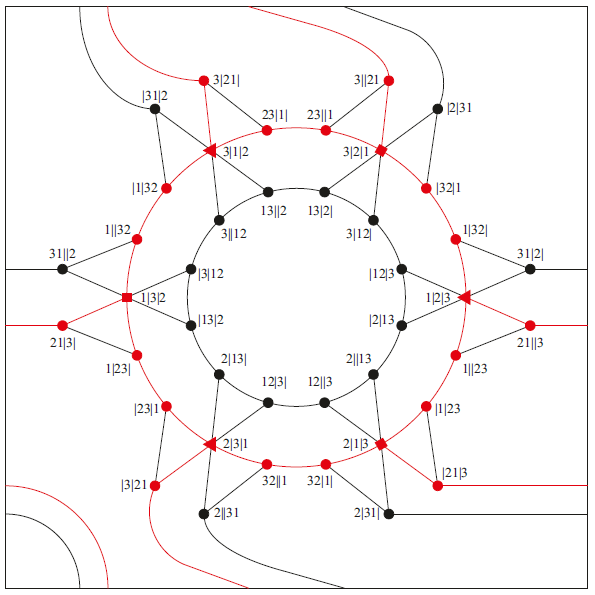
\includegraphics[width=190pt]{../img/tolgraph-O^3_222-subdivision.png}
        \caption{Rdeči podgraf grafa $L_{222}^3$ je subdivizija grafa $K_{3,3}$.}
    \end{figure}
\end{frame}

\begin{frame}{Simetrije}
    TODO
\end{frame}

\section{Oxfordski graf}
\begin{frame}{Oxfordski graf}
    \alert{Oxfordski graf} je poseben primer londonskega grafa, kjer velja, da so vse palice velikosti $n$, pri čemer je $n$ število krogel. Oxfordski graf označimo z $O^n_p$, zanj torej velja $O^n_p := L^n_{n^p}$.
    
\end{frame}

\begin{frame}{Lastnosti}
    \begin{block}{Trditev}
           Število vozlišč oxfordskega grafa $O^n_p$ je enako \[\frac{(n+p-1)!}{(p-1)!}.\]
    \end{block}    
    \begin{block}{Trditev}
        Število povezav oxfordskega grafa $O^n_p$ je enako
        \[ \frac{np}{2} \frac{(p-2+n)!}{(p-2)!} .\]
    \end{block}
    

\end{frame}

\begin{frame}{Dokaz formule za število povezav oxfordskega grafa}
    \begin{block}{Lema o rokovanju}
        Za vsak graf $\graf$ velja formula
        \begin{equation*}
        \sum_{u \in V(G)}\!\! \stopnja u = 2 \cdot |E(G)|.
        \end{equation*}
    \end{block}
    
    Spomnimo se še, da velja formula 
    \[ {b+w \choose l} = \sum_{k=0}^{l}{b \choose k}{w \choose l-k} \]
\end{frame}

%\section{Uporaba}
%\begin{frame}{Primeri uporabe}
%    \begin{itemize}
%        \item Problem londonskega stolpa je bil razvit z namenom merjenja sposobnosti načrtovanja in reševanja problemov pri bolnikih s poškodbami čelnega režnja možganov.
%        \item Slabo reševanje londonskega stolpa se interpretira kot nezmožnost učinkovitega načrtovanja.
%        \item Uporabljen je bil za ocenjevanje napredka bolezni pri bolnikih z Alzheimerjevo in Parkinsonovo boleznijo.
%        \item Uporabljen je bil tudi za opazovanje vedenja majhnih otrok pri reševanju problemov.
%    \end{itemize}
%\end{frame}

\end{document}
